\documentclass[a4paper]{report}
\usepackage{vntex}
%\usepackage[english,vietnam]{babel}
%\usepackage[utf8]{inputenc}

%\usepackage[utf8]{inputenc}
%\usepackage[francais]{babel}
\usepackage{a4wide,amssymb,epsfig,latexsym,multicol,array,hhline,fancyhdr}
\usepackage{booktabs}
\usepackage{amsmath}
\usepackage{lastpage}
\usepackage[lined,boxed,commentsnumbered]{algorithm2e}
\usepackage{enumerate}
\usepackage{color}
\usepackage{graphicx}							% Standard graphics package
\usepackage{array}
\usepackage{tabularx, caption}
\usepackage{multirow}
\usepackage[framemethod=tikz]{mdframed}% For highlighting paragraph backgrounds
\usepackage{multicol}
\usepackage{rotating}
\usepackage{graphics}
\usepackage{geometry}
\usepackage{setspace}
\usepackage{epsfig}
\usepackage{tikz}
\usepackage{listings}

\usetikzlibrary{arrows,snakes,backgrounds}
\usepackage{hyperref}
\hypersetup{urlcolor=blue,linkcolor=black,citecolor=black,colorlinks=true} 
%\usepackage{pstcol} 								% PSTricks with the standard color package

\newtheorem{theorem}{{\bf Định lý}}
\newtheorem{property}{{\bf Tính chất}}
\newtheorem{proposition}{{\bf Mệnh đề}}
\newtheorem{corollary}[proposition]{{\bf Hệ quả}}
\newtheorem{lemma}[proposition]{{\bf Bổ đề}}

\everymath{\color{blue}}
%\usepackage{fancyhdr}
\setlength{\headheight}{40pt}
\pagestyle{fancy}
\fancyhead{} % clear all header fields
\fancyhead[L]{
 \begin{tabular}{rl}
    \begin{picture}(25,15)(0,0)
    \put(0,-8){
\includegraphics[width=8mm, height=8mm]{hcmut.png}}
    %\put(0,-8){\epsfig{width=10mm,figure=hcmut.eps}}
   \end{picture}&
	%
\includegraphics[width=8mm, height=8mm]{hcmut.png} & %
	\begin{tabular}{l}
		\textbf{\bf \ttfamily Trường Đại Học Bách Khoa Tp.Hồ Chí Minh}\\
		\textbf{\bf \ttfamily Khoa Khoa Học và Kỹ Thuật Máy Tính}
	\end{tabular} 	
 \end{tabular}
}
\fancyhead[R]{
	\begin{tabular}{l}
		\tiny \bf \\
		\tiny \bf 
	\end{tabular}  }
\fancyfoot{} % clear all footer fields
\fancyfoot[L]{\scriptsize \ttfamily Luận văn tốt nghiệp đại học - 2014/2018}
\fancyfoot[R]{\scriptsize \ttfamily Trang {\thepage}/\pageref{LastPage}}
\renewcommand{\headrulewidth}{0.3pt}
\renewcommand{\footrulewidth}{0.3pt}


%%%
\setcounter{secnumdepth}{4}
\setcounter{tocdepth}{3}
\makeatletter
\newcounter {subsubsubsection}[subsubsection]
\renewcommand\thesubsubsubsection{\thesubsubsection .\@alph\c@subsubsubsection}
\newcommand\subsubsubsection{\@startsection{subsubsubsection}{4}{\z@}%
                                     {-3.25ex\@plus -1ex \@minus -.2ex}%
                                     {1.5ex \@plus .2ex}%
                                     {\normalfont\normalsize\bfseries}}
\newcommand*\l@subsubsubsection{\@dottedtocline{3}{10.0em}{4.1em}}
\newcommand*{\subsubsubsectionmark}[1]{}
\makeatother

\definecolor{dkgreen}{rgb}{0,0.6,0}
\definecolor{gray}{rgb}{0.5,0.5,0.5}
\definecolor{mauve}{rgb}{0.58,0,0.82}
\lstset{frame=tb,
	language=Matlab,
	aboveskip=3mm,
	belowskip=3mm,
	showstringspaces=false,
	columns=flexible,
	basicstyle={\small\ttfamily},
	numbers=none,
	numberstyle=\tiny\color{gray},
	keywordstyle=\color{blue},
	commentstyle=\color{dkgreen},
	stringstyle=\color{mauve},
	breaklines=true,
	breakatwhitespace=true,
	tabsize=3,
	numbers=left,
	stepnumber=1,
	numbersep=1pt,    
	firstnumber=1,
	numberfirstline=true
}

\renewcommand{\chaptername}{Chương}
\renewcommand\bibname{Tài liệu tham khảo}
\usepackage[toc,page]{appendix}
\usepackage{indentfirst}
\usepackage{subfig}
\usepackage{wrapfig}

\begin{document}

\begin{titlepage}
\begin{center}
ĐẠI HỌC QUỐC GIA THÀNH PHỐ HỒ CHÍ  \\
TRƯỜNG ĐẠI HỌC BÁCH KHOA \\
KHOA KHOA HỌC - KỸ THUẬT MÁY TÍNH 
\end{center}

\vspace{1cm}

\begin{figure}[h!]
\begin{center}

\includegraphics[width=3cm]{hcmut.png}
\end{center}
\end{figure}

\begin{center}
\begin{tabular}{c}
	\multicolumn{1}{c}{\textbf{{\Huge LUẬN VĂN TỐT NGHIỆP}}}\\
	~~\\
	\\
	\\
	\hline
	\\
	\multicolumn{1}{l}{\textbf{{\huge Nghiên cứu giải thuật xử lý ảnh}}}\\
	\\
	
	\textbf{{\huge \& Giải pháp Egde Computing tổng thể}}\\
	\\
	\hline
\end{tabular}
\end{center}

\vspace{3cm}

\begin{table}[h]
\begin{tabular}{rrll}
\hspace{5 cm} & GVHD: &TS. LÊ THÀNH SÁCH&\\
& & PGS.TS THOẠI NAM\\
& & \\	
& SV: & Trần Minh Thông & 1413843\\
& & Hồ Bảo Quốc & 1413171 \\
& & Dương Viết Trung & 1414272\\

\end{tabular}
\end{table}

\begin{center}
{\footnotesize TP.HỒ CHÍ MINH, THÁNG 4/2017}
\end{center}
\end{titlepage}


\thispagestyle{empty}

\newpage
\begin{center}
	\textbf{LỜI CAM ĐOAN}
\end{center}

Luận văn của chúng tôi có tham khảo các tài liệu, bài báo, trang web được trình bày ở
mục tài liệu tham khảo và ở mỗi tham khảo chúng tôi đều trích dẫn nguồn gốc. Chúng tôi
xin cam đoan rằng ngoài các trích dẫn từ các tham khảo trên toàn bộ nội dung trong báo cáo
là do chúng tôi tự soạn thảo từ kết quả thực hiện của riêng chúng tôi, không sao chép từ
bất kì tài liệu nào khác.\\

Chúng tôi sẽ hoàn toàn chịu xử lí theo quy định nếu có bất cứ sai phạm nào so với lời
cam kết.

\newpage 
\begin{center}
	\textbf{LỜI CẢM ƠN}
\end{center}

Đầu tiên, nhóm xin gửi lời cảm ơn chân thành đến thầy hướng dẫn TS. Lê Thành Sách
đã luôn trao đổi, góp ý và hướng dẫn chúng tôi trong suốt thời gian qua. Thầy không những
chia sẻ những kiến thức liên quan đến nội dung đề tài mà còn giúp đỡ, định hướng các công 
việc cần thiết và đốc thúc chúng tôi hoàn tất luận văn tốt nghiệp của mình.\\

Xin cảm ơn chân thành PGS.TS Thoại Nam, người đã định hướng đề tài và tin tưởng giao đề 
tài rất hay và thiết thực này cho nhóm. Thầy cũng là người cung cấp thiết bị cũng như 
những sự hỗ trợ cần thiết khác cho nhóm, giúp nhóm có cơ sở để hoàn thành bài tốt nghiệp
 của mình. \\

Xin gửi lời cảm ơn hai anh khóa trên là Minh và Thành  đã chỉ dẫn và hỗ trợ các kiến thức
cùng công cụ nền tảng cần thiết để hiện thực và thử nghiệm chương trình.\\

Xin chân thành cảm ơn đến các thầy cô trường Đại học Bách Khoa thành phố Hồ Chí
Minh và đặc biệt là khoa Khoa học và Kĩ thuật Máy tính đã giảng dạy những kiến thức bổ
ích cho chúng tôi trong suốt thời gian học tại trường.\\

Cuối cùng, chúng tôi gởi lời cảm ơn tới các bạn, người thân đã tham gia giúp đỡ nhóm tạo
nên bộ dữ liệu huấn luyện cho chương trình.\\


\newpage
\begin{center}
	\textbf{TÓM TẮT LUẬN VĂN}
\end{center} 

Trong vài năm trở lại đây, chứng kiến sự bùng nổ của mạng nơ-ron nhân tạo hay phương pháp 
học sâu đã đạt được những thành tựu vượt bậc, đặc biệt trong ngành thị giác máy tính. Các 
ứng dụng của thị giác máy tính len lỏi trong mọi lĩnh vực đời sống của xã hội, nổi bật là 
các ứng dụng tìm kiếm nội dung ảnh, bản đồ, các ứng dụng trong y học, xe tự lái, .. Các ứng
 dụng này đều được xây dựng trên cái bài toán nhỏ hơn như phân loại ảnh (classification), 
 định vị (localization) và phát hiện đối tượng (detection), phân mảnh đối tượng 
 (segmentation).  Trong phạm vi luận văn này, nhóm ưu tiên tìm hiểu bài toán phát hiện
đối tượng, là sự kết hợp giữa hai bài toán định vị đối tượng và phân loại ảnh, sử dụng
phương pháp học sâu.  Cuộc thi nổi tiếng nhất cho bài toán nhận dạng đối tượng là ILSVRC, 
có rất nhiều mô hình dẫn đầu xuất phát từ cuộc thi này. Đặc biệt là mô hình SSD, giành 
chiến thắng cuộc thi ILSVRC \\

Mạng nơ-ron sâu thực chất không phải là một khái niệm mới, mà nó xuất hiện từ những
năm 19xx. Lý do khiến chúng mãi bây giờ mới nổi lên, chính là vì sự lớn nhanh của sức
mạnh phần cứng máy tính cùng trong thời đại bùng nổ về dữ liệu. Các mạng nơ-ron sâu 
đòi hỏi khả năng tính toán vô cùng lớn của phần cứng để tính toán hàng gigabyte,
terabyte dữ liệu. Phần cứng máy tính hiện nay không chỉ có đột phá về sức mạnh tính 
toán mà còn về kích thước của chúng. Hiện nay đã có những máy tính có sức mạnh trung
bình có kích thước chỉ bằng một thẻ bài tây, chính ưu điểm này mở đường cho một xu
hướng mới, tính toán ở cạnh mạng - edge computing, thiết bị tính toán được cài đặt
ngay trên thiết bị quan trắc dữ liệu giúp tối ưu đường truyền, giảm tải cho server,
ận dụng khả năng tính toán. Tuy nhiên, vẫn còn đó những cơ hội cũng như thách thức
đang chờ được giải quyết. Trong phạm vi luận văn, nhóm đã triển khai giải thuật 
phát hiện đối tượng lên thiết bị IoT của Nvidia là Jetson Tx2. 

\newpage
\begin{center}
	\textbf{BỐ CỤC LUẬN VĂN}
\end{center} 

Luận văn gồm 3 phần chính, phần mở đầu, phần hiện thực và kết luận \\

Phần mở đầu được nêu trong CHƯƠNG 1: GIỚI THIỆU, nhằm cung cấp cái nhìn tổng quan về đề tài,
 mục tiêu của nhóm cũng như quá trình nghiên cứu, thực hiện luận văn của nhóm.\\

Phần hiện thực gồm 4 chương\\
\begin{itemize}
	\item CHƯƠNG 2: KIẾN THỨC NỀN TẢNG. Trình bày kiến thức cơ sở của bài toán phát hiện
	 đối tượng, ưu điểm của hướng tiếp cận sử dụng mạng nơ-ron tích chập. Một số bài 
	 toán và mô hình liên quan trực tiếp tới bài toán phát hiện đối tượng. Trình bày 
	 những kiến thức cơ bản về tính toán cạnh mạng, các thông số cần biết của thiết bị
	  và nêu lên những cơ hội cũng như khó khăn còn tồn tại của tính toán mạng. 
	\item CHƯƠNG 3: CÁC CÔNG TRÌNH LIÊN QUAN. Trình bày một số một hình liên quan 
	trực tiếp và được sử dụng trong luận văn, chủ yếu là mô hình ssd và các biến thể 
	của nó.

	\item CHƯƠNG 4: NỘI DUNG THỰC HIỆN
\end{itemize}

Phần kết luận là chương cuối cùng, CHƯƠNG 5: KẾT LUẬN, ĐÁNH GIÁ, HƯỚNG PHÁT TRIỂN. Tại đây, nhóm xin đưa
ra một số nhận xét về công trình nghiên cứu của mình, cũng như những đóng góp mà luận
văn đem lại. Bên cạnh đó, nhóm nhìn nhận lại những sai sót và đưa ra những hướng giải
quyết, phát triển trong tương lai.\\

Ngoài 3 phần chính vừa nêu trên, luận văn còn bao gồm N phụ lục bổ sung thêm các
thông tin cần thiết nhằm hỗ trợ các nhóm phát triển sau. Cụ thể:
\begin{itemize}
	\item PHỤ LỤC 1:
\end{itemize}

\newpage %danh muc bang
\listoftables
\newpage
\listoffigures


\newpage
\tableofcontents
\newpage

%%%%%%%%%%%%%%%%%%%%%%%%%%%%%%%%%


%%%%%%%%%%%%%%%%%%%%%%%%%%%%%%%%%
\chapter{GIỚI THIỆU} 
Trí tuệ nhân tạo đang là lĩnh vực đang được quan tâm hàng đầu hiện nay,
không chỉ thu hút sự quan tâm của đông đảo các nhà khoa học, mà các tập đoàn
công nghệ lớn cũng tham gia tích cực vào nghiên cứu và ứng dụng trí tuệ vào các
mảng của đời sống. Trí tuệ nhân tạo đang dần đi vào thực tiễn đời sống và ngày
càng gần gũi với con người, nó giúp nâng cao chất lượng cuộc sống, giúp con người
lao động, thay thế con người làm việc ở những môi trường nguy hiểm,.. Ở một
khía cạnh nào đó, trí tuệ nhân tạo sẽ là tương lai của loài người.\\

Trong phần thứ nhất của luận văn, nhóm sẽ 
trình bày nguyên nhân nhóm chọn đề tài cũng như mục tiêu mà nhóm mong muốn đạt được 
khi thực hiện đề tài.

\section{Lý do chọn đề tài}

	Trong những năm gần đây, những nghiên cứu về deep learning đang thu được
những kết quả ấn tượng, đặc biệt trong lĩnh vực thị giác máy tính, các mô 
hình deep learning thu được kết quả có độ chính xác cao hơn và có nhiều ưu 
điểm vượt trội so với các
phương pháp thị giác máy tính truyền thống. Chúng đã đưa các công nghệ tương lai
 như xe tự lái, hệ thống giám sát theo dõi qua video, nhận diện khuôn mặt, .. đến 
 gần với hiện thực hơn, hiệu quả hơn và thậm chí một số công nghệ đã được áp dụng 
 thành công trong một số điều kiện nhất định. Sự thành công đã được kiểm chứng và 
 tiềm năng to lớn của deep learning, nhóm mong muốn có thể áp dụng những giải thuật, 
 những mô hình hiện có và tìm cách cải tiến nó để giải quyết những vấn đề thực tế ở Việt Nam hiện nay. \\
 
 Cuối năm 2017, phóng viên của đài BBC đã thực hiện một đoạn phóng sự về hệ thống giám sát qua video tại thành phố Quý Dương,
 của Trung Quốc \footnote{https://www.bbc.com/news/av/world-asia-china-42248056/in-your-face-china-s-all-seeing-state}, hệ thống này sử dụng một mạng lưới dày 
 đặc các camera được tích hợp trí tuệ nhận tạo và xây dựng một cơ sở dữ liệu của người dân thành phố. Trong phóng sự, hệ thống 
 này sau khi nhập dữ liệu mới là nhân dạng khuôn mặt của phóng viên BBC, thì nó cần hơn 7
  phút để tìm ra vị trí của phóng viên trong thành phố. Đây là một trong nhiều ứng dụng đáng kinh ngạc 
  của trí tuệ nhân tạo. Sự mới mẻ mang tính đột phá chính là động lực cho nhóm thực hiện đề tài này.\\

%-------------Figure 2 ---------------------------------
%\begin{figure}[h!]
%\centering
%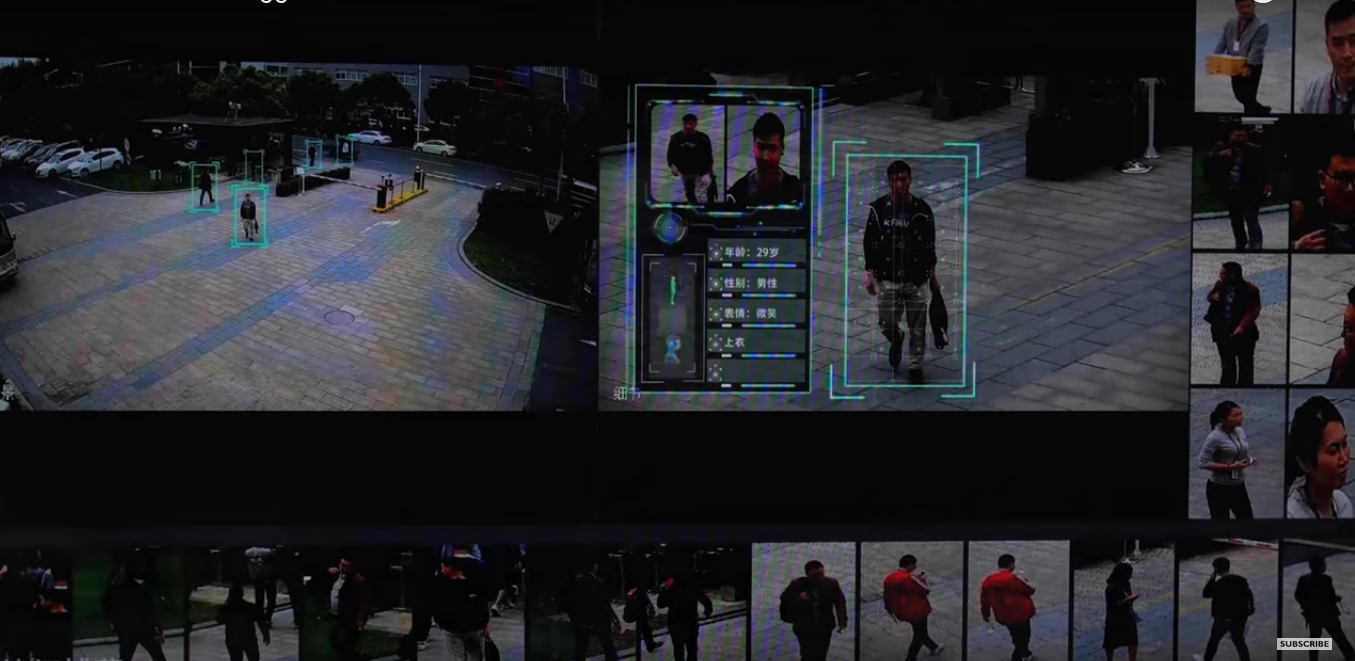
\includegraphics[width=0.8\textwidth]{1_01.png}
%\caption{Những nhà quản lý cho rằng hệ thống có khả năng so khớp khuôn mặt với chứng từ, ước lượng tuổi, dân tộc, giới tính}
%\end{figure}


\begin{figure}[h] \label{fig:three-alternative-operations}
	\centering
	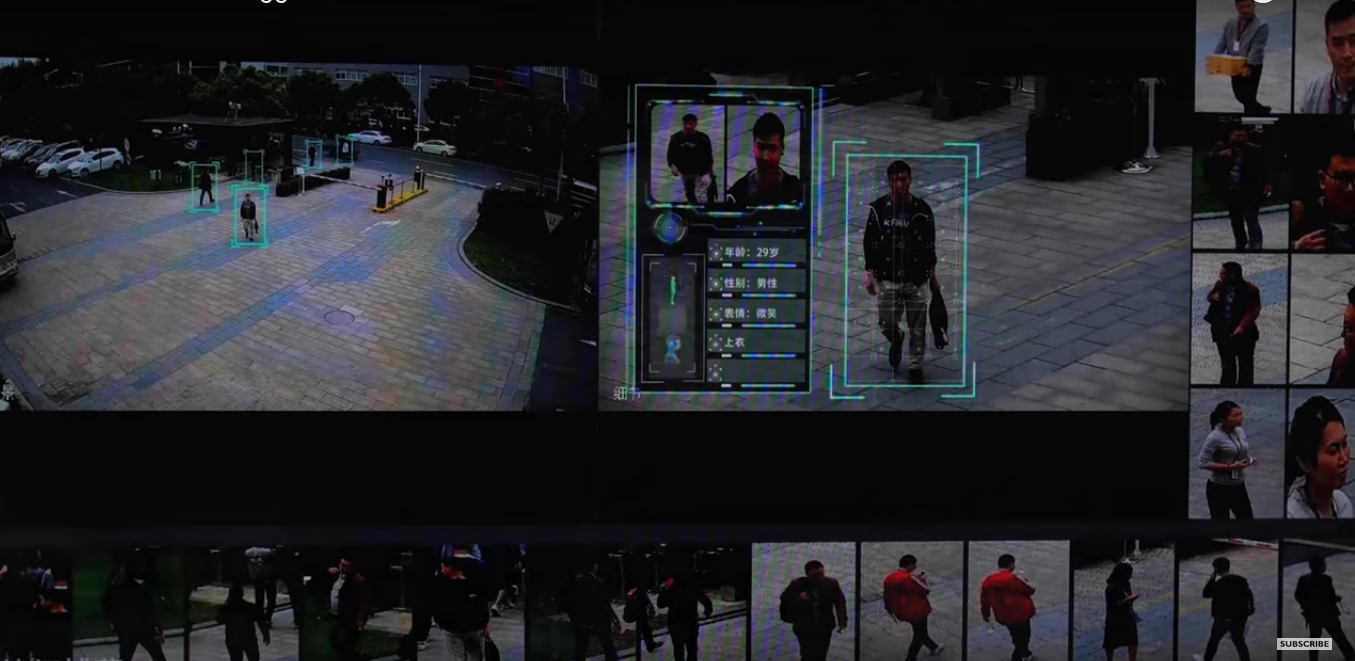
\includegraphics[width=0.9\textwidth]{1_01.png}\\
	Hình a\\
	\color{black}
	%\captionsetup{width=.8\textwidth}
	\begin{tabular}{cc}
		\\
		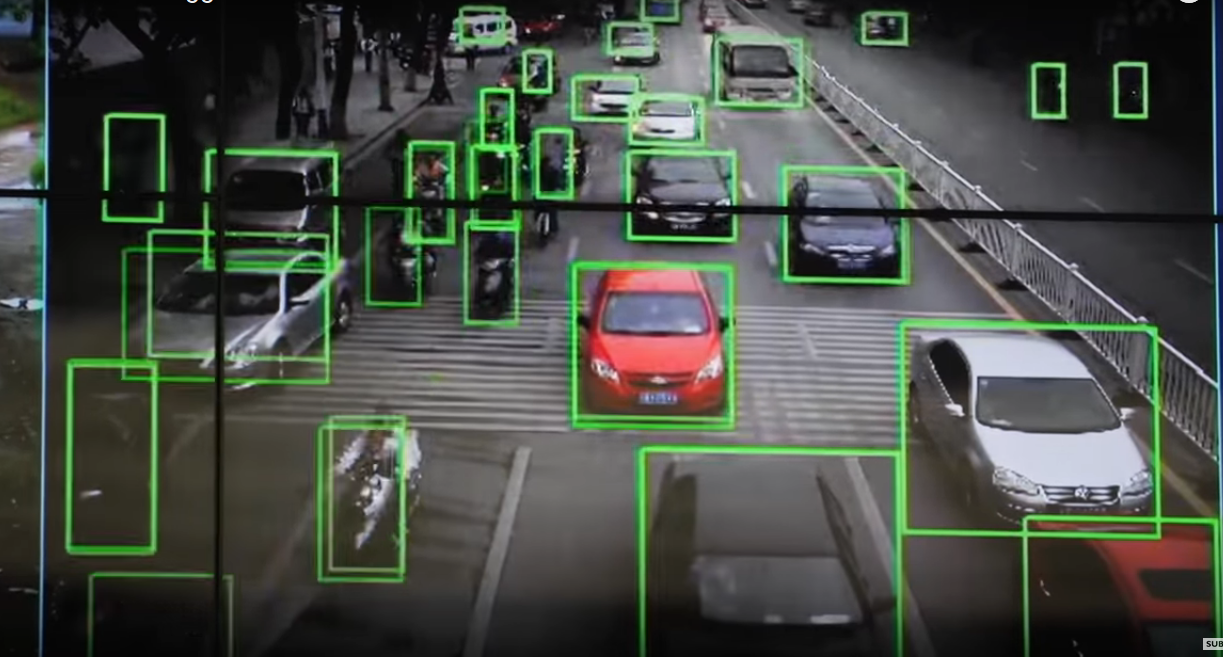
\includegraphics[width=0.5\textwidth]{1_02.png} &
		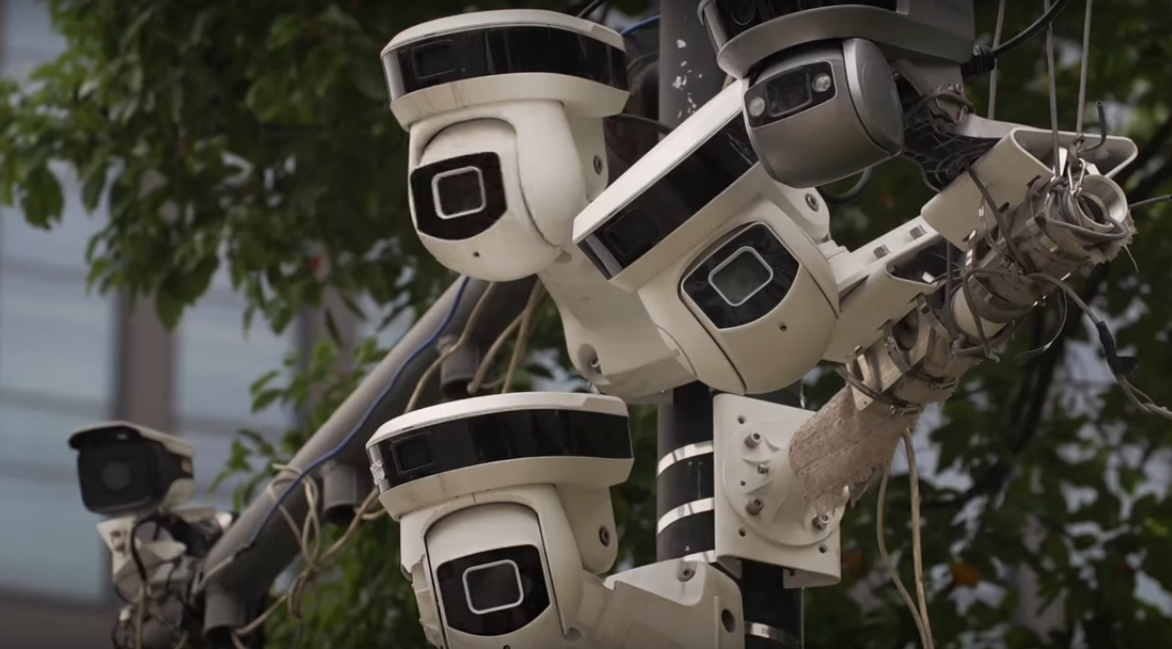
\includegraphics[width=0.49\textwidth]{1_03.png} \\
		
		Hình b & Hình c
	\end{tabular}

	\caption{Hệ thống giám sát video được trải khai tại Trung Quốc} Nhà quản lý của hệ thống này cho rằng có khả năng so khớp khuôn mặt với
	chứng từ cá nhân, dự đoán tuổi, giới tính và dân tộc (Hình a). Hệ thống còn có khả năng theo dõi xe hơi của người dân qua biển số (Hình b). 
	Một vị trí được gắn camera tích hợp trí tuệ nhân tạo dày đặc (Hình c) 
	\footnote{ Hình ảnh được trích xuất từ video https://www.bbc.com/news/av/world-asia-china-42248056/in-your-face-china-s-all-seeing-state}
\end{figure}	
\footnotetext[1]{avc}
\section{Tính thực tiễn}
Một số vấn đề thực tế và khả năng ứng dụng của đề tài: \footnote[3]{text}
\begin{itemize}
\item Phát hiện ngủ gật. Hằng năm ở nước ta vẫn tồn tại những vụ tai nạn thương tâm xảy 
ra do tài xế ngủ gật, khi tìm kiếm với từ khóa "tai nạn do ngủ gậc" Google trả về  gần 3 triệu kết 
quả trong hơn nửa giây hay số lượng lớn bài báo liên quan tới ngủ gậc khi tìm kiếm trên 
báo trực tuyến tuoitre.vn (Hình \ref{drowsiness}.a) . Một hệ thống phát hiện trạng thái của lái xe có thể giảm thiểu khả 
năng xảy tai nạn thảm khốc hằng năm. Một hệ thống được lắp đặt trên xe và đủ thông minh 
để xử lí các tình huống khác nhau ở trong các điều kiện khác nhau trong thực tế. 

\item Tìm kiếm nội dung trong video. Ứng dụng này liên quan tới việc giải các bài toán 
phân loại (classification), phát hiện đối tượng (object detection), theo vết (tracking) hay đếm (counting).
Giả sử có thể xây dựng một hệ thống giám sát trong các trung tâm thương mại, các khu chung cư lớn, 
có khả năng theo dõi đặc điểm của con người như giới tính, các phụ kiện thời trang đi kèm như túi xách, balo, ..,
có đeo kính mắt, có đội mũ hay không? Ứng dụng đầy hứa hẹn khi tìm kiếm người có đặc điểm được mô tả 
hay, tìm kiếm những đứa trẻ đi lạc trong trung tâm thương mại, hay cảnh báo an ninh cho các tổ chức tài
chính, ngân hàng. 

\item Giám sát giao thông. 
\footnotetext[1]{Hình ảnh từ http://tuoitre.vn}
\footnotetext[2]{Hình ảnh từ https://thenextweb.com/artificial-intelligence/2018/03/23/affectivas-automotive-ai-could-keep-distracted-and-drowsy-drivers-from-causing-accidents/}
\end{itemize}

\begin{figure}[h] 
	\centering
	\color{black}
	%\captionsetup{width=.8\textwidth}
	\begin{tabular}{cc}
		\\
		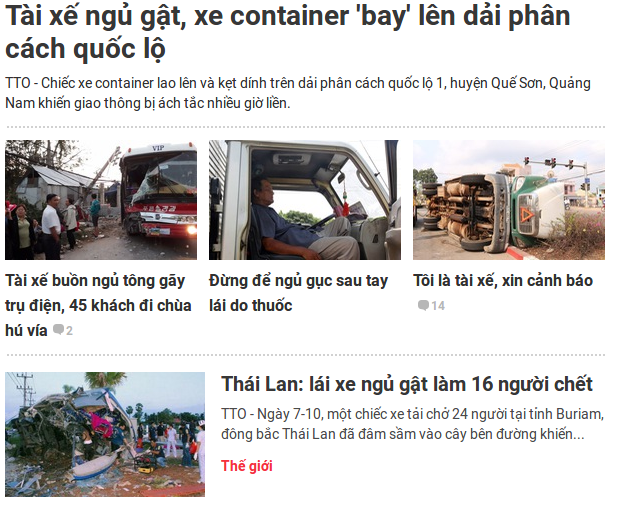
\includegraphics[width=0.5\textwidth]{1_04.png} &
		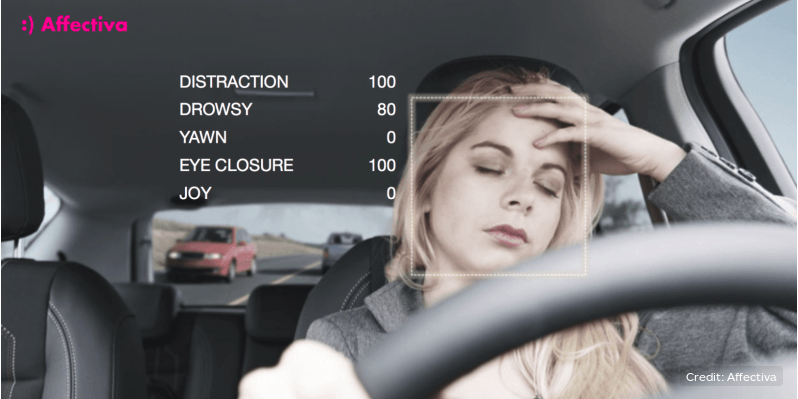
\includegraphics[width=0.49\textwidth]{1_06.png} \\
		
		Hình a \footnote[1]{Hình ảnh từ http://tuoitre.vn} & 
		Hình b \footnote[2]{Hình ảnh từ https://thenextweb.com/artificial-intelligence/2018/03/23/affectivas-automotive-ai-could-keep-distracted-and-drowsy-drivers-from-causing-accidents/}
	\end{tabular}

	\caption{Tình trạng ngủ gậc \& Mô phỏng hệ thống phát hiện ngủ gậc}
	\label{drowsiness}
\end{figure}	

%------------- example of video surveilances ---------------------------------
\begin{figure}[h!]
\centering
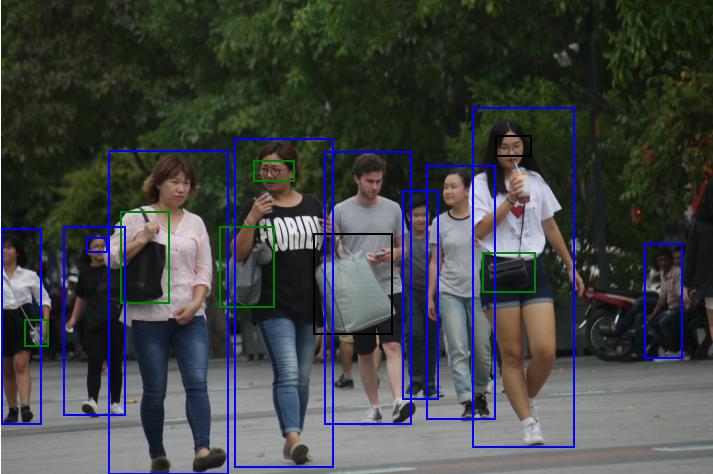
\includegraphics[width=0.8\textwidth]{1_05.png}
\caption{Một ví dụ về giám sát, nhận dạng đặc điểm con người}
\end{figure}

\section{Mục tiêu của luận văn}
Hai nhiệm vụ của luận văn được đặc ra bao gồm:
\begin{itemize}
\item Thử nghiệm và tìm cách cải tiến mô hình SSD, khắc phục nhược điểm của mô hình SSD là khả năng phát hiện đối tượng có kích thước nhỏ.
\item Triển khai hệ thống đã thử nghiệm lên board Jetson TX2.
\end{itemize} 

\section{Quy trình thực hiện luận văn}
Quá trình thực hiện đề tài gồm các bước chính sau: 
\begin{itemize}
	\item  Bước 1: Tìm hiểu và phân tích đề tài, đưa ra các vấn đề chính cần giải quyết
	\item  Bước 2: Nghiên cứu, tìm hiểu các phương pháp, thuật toán có thể áp dụng vào đề tài.
	\item  Bước 3: Tìm kiếm các tập dữ liệu có sẵn và tự xây dựng tập dữ liệu mới, chỉnh sửa và rút trích những thông tin cần thiết để sử dụng cho quá trình huấn luyện và kiểm thử. 
	\item  Bước 4: Thực hiện kiểm thử và đưa ra đánh giá, lặp lại bước 2
	\item  Bước 5: Đề xuất phương pháp cải tiến, hiện thực và đánh giá ưu điểm, nhược điểm của phương pháp.
\end{itemize} 

\chapter{KIẾN THỨC NỀN TẢNG}
Chương này sẽ tập trung trình bày các kiến thức nền tảng, quá trình phát triển của bài 
toán phát hiện đối tượng, ưu điểm của giải pháp deep learning so với phương pháp thị giác 
máy tính truyền thống. Đồng thời chương này cũng cung cấp những cơ hội và thách thức mà 
điện toán cạnh mạng mang lại. 

\section{Kiến thức xử lý ảnh}
\subsection{Bài toán phát hiện đối tượng}
Về cơ bản, một hệ thống Phát hiện đối tượng sẽ nhận đầu vào là một bức ảnh chưa qua xử lý, 
và đầu ra là kết quả các hộp biên bao quanh đối tượng và xác suất phân loại đối tượng đó 
thuộc lớp nào. Như đã trình bày ở phần giới thiệu, bài toán phát hiện đối tượng là sự kết
hợp hai bài toán định vị đối tượng (localization) bằng cách vẽ các hộp biên thích hợp bao 
quanh đối tượng sau đó thực hiện phân loại (classification) các đối tượng này. Điều này đòi 
hỏi hệ thống thực hiện tác vụ phức tạp hơn so với các hệ thống truyền thống chỉ thực hiện
chức năng phân loại ảnh. 

\subsection{Phương pháp thị giác máy tính truyền thống}
\subsubsection{Adaboost}
\subsubsection{HOG}

\subsection{Phương pháp học sâu}
\subsubsection{R-CNN}
R-CNN là tiền thân của mạng Faster R-CNN. \\

R-CNN (Region-based Convolutional Neural Network, 2014), gồm 3 bước:
\begin{enumerate}
    \item Dùng giải thuật Selective Search quét ảnh đầu vào các vùng có thể chứa đối tượng. (generating ~2000 region proposals)
    \item Cho các vùng dự đoán qua một mạng CNN
	\item Lấy đầu ra của các CNN ở bước 2:
	\begin{enumerate}
        \item Làm đầu vào của một bài toán phân loại SVM
        \item Làm đầu vào của một linear regressor to tighten the bb of the object, if such an object exists.
	\end{enumerate}
\end{enumerate}

Một mạng R-CNN được mô tả như hình.
%------------- example of video surveilances ---------------------------------
\begin{figure}[h!]
	\centering
	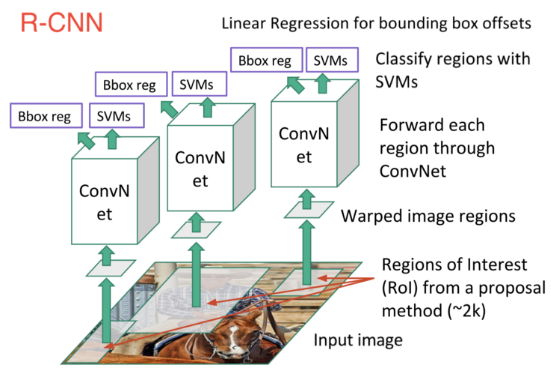
\includegraphics[width=0.7\textwidth]{2_rcnn.png}
	\caption{Mô phỏng một mạng R-CNN \cite{detectionoverview}}
	\end{figure}

Đầu tiên, dự đoán các vùng có thể chứa object (propose regions), trích xuất các đặc trưng
và phân loại các vùng dự đoán dựa trên các đặc trưng của chúng. Về bản chất, bài toán thực
chất là bài toán phân loại truyền thống. R-CNN rất trực quan nhưng rất chậm và kết quả 
không tối ưu. (Chậm vì phải chạy thuật toán Selective Search, mỗi propose regions phải 
qua một lớp CNN, SVMs khá phức tạp với bài toán phân loại n lớp. Do quá trình propose 
regions và trích xuất đặc trưng tách biệt với nhau, nên kết quả học không được tối ưu, 
điều này sẽ được giải thích kỹ hơn ở các mô hình tiếp theo).

\subsubsection{Fast R-CNN}
Fast R-CNN cải thiện tốc độ của R-CNN bằng hai thay đổi chính:

\begin{enumerate}
	\item Thực hiện trích xuất đặc trưng trên bức ảnh trước khi dự đoán vùng chứa đối tượng, 
do đó nó chỉ cần một bước CNN cho toàn bộ bức ảnh thay vì hơn 2000 bước CNN tương ứng với 2000 vùng dự đoán như R-CNN.
	\item  Thay thế SVM bằng lớp softmax. Thực chất SVM là một mô hình phân loại n class, 
với softmax chỉ cần thêm vào mô hình hiện tại thay vì tạo một mô hình phân loại như SVM.   
\end{enumerate}

%------------- example of fast rcnn---------------------------------
\begin{figure}[h!]
	\centering
	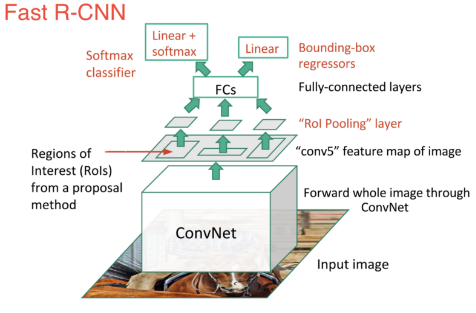
\includegraphics[width=0.7\textwidth]{2_fast.png}
	\caption{Mô phỏng một mạng Fast R-CNN \cite{detectionoverview}}
\end{figure}

Như hình minh họa, các vùng được dự đoán chứa các đối tượng sẽ được sinh ra dựa vào 
feature map cuối cùng của lớp CNN, không phải từ ảnh gốc như R-CNN. Kết quả là chỉ cần 
uấn luyện một lớp CNN cho toàn bộ bức ảnh. \\

Một điểm khác biệt khác, thay vì huấn luyện một mô hình phân loại SVM cồng kềnh thì 
việc sử dụng một lớp softmax giúp tính toán ra trực tiếp xác suất phân loại của mỗi lớp. 
Lúc này, chỉ cần phải huấn luyện một mạng CNN thay vì nhiều mạng CNN và mô hình phân loại 
SVM. \\

Fast R-CNN đã khắc phục được nhược điểm về tốc độ của R-CNN. Nhưng vẫn còn tồn tại một
 "nút thắt cổ chai" trong Fast R-CNN đó là thuật toán selective search phát hiện các 
 vùng dự đoán. 

\subsubsection{Faster R-CNN}
%\subsubsection{FCN}
Faster R-CNN hướng đến việc giải quyết yếu điểm của Fast R-CNN là giải thuật selective
 search. Faster R-CNN thay giải thuật selective search bằng một mạng RPN (Region Proposal
 Network).\\

 %%% sliding window %%%%
\begin{wrapfigure}{r}[0pt]{0.5\linewidth}
	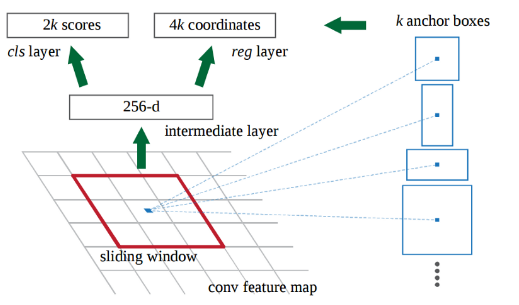
\includegraphics[scale=0.45]{2_slide.png}
	\caption{caption thôi \cite{detectionoverview}}
\end{wrapfigure}

RPN thực hiện như sau:
\begin{itemize}
\item Tại lớp cuối cùng của CNN ban đầu, dịch chuyển một cửa sổ trượt có kích thước 3x3 
trên toàn bộ feature map và ánh xạ vào một lớp có kích thước nhỏ hơn. (256-d)
\item Tại mỗi vị trí trên feature map, nó sinh ra  k vùng dự đoán hay các anchor boxes (default bouding box)
\item Mỗi vùng dự đoán bao gồm: điểm của đối tượng (objectness score - tỉ lệ xuất hiện của đối tượng trong bounding box) cho vùng đó và 4 tham số cx, cy, w, h biểu diễn cho bounding box.
\end{itemize}

Nói cách khác, tại mỗi vị trí (location) trong feature map cuối cùng, xét k bounding box 
có hình dạng khác nhau: box cao, dài, rộng, vuông, ...Mỗi box có 5 tham số, 4 tham số thể 
hiện tọa độ của bounding box, tham số còn lại thể hiện trong bounding box có chứa đối 
tượng hay không.\\

\begin{figure}[h!]
	\centering
	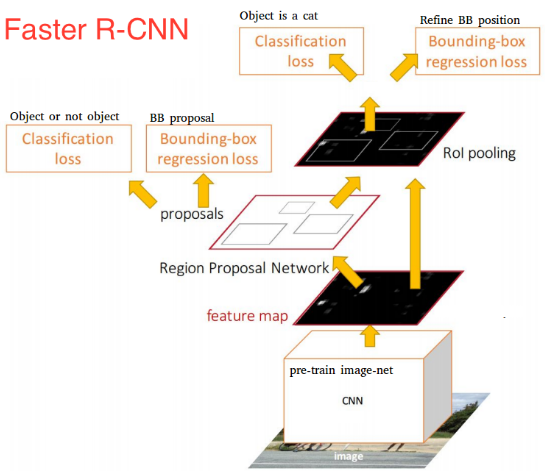
\includegraphics[width=0.7\textwidth]{2_faster.png}
	\caption[Caption for LOF]{Mô phỏng một mạng Faster R-CNN \cite{detectionoverview}} 
\end{figure}

Trong hình (), 2k score thể hiện xác suất bounding box chứa đối tượng của k bounding box.
Lưu ý rằng RPN chỉ xuất ra tọa độ của bounding box, vai trò của nó vẫn là đưa ra các vùng 
dự đoán (propose regions), chứ không cố gắng thực hiện phân loại các đối tượng nằm trong 
vùng đó. Nếu anchor box có tỉ lệ xuất hiện đối tượng (objectness score) lớn hơn một ngưỡng 
nào đó, thì tọa độ anchor box đó là sẽ là vùng dự đoán cần tìm (region proposal). \\
 
Khi đã có tìm được các vùng dự đoán, đó chính là đầu vào của mạng Fast R-CNN. Từ mạng 
Fast R-CNN, thêm vào các lớp pooling, các lớp fully-connected, và cuối cùng là lớp softmax
 và bounding box regressor. Tóm lại, Faster R-CNN = RPN + Fast R-CNN.\\

 
Faster R-CNN nhanh hơn và chính xác hơn so với Fast R-CNN hay trước đó là R-CNN
 nhưng đều sử dụng một triết lý thiết kế chung, đó là sinh ra các vùng dự đoán 
 trước, sau đó thực hiện phân loại các vùng dự đoán này. Nhưng so với các mạng 
 ra đời sau, Faster R-CNN vẫn còn phức tạp và chưa đáp ứng được yêu cầu về thời gian thực. 

\subsection{Một số mô hình xử lý hợp nhất}
\subsubsection{SSD}
Single Shot Detector, có tốc độ gấp nhiều lần Faster R-CNN. \\

Các mô hình ở trên đều thực hiện dự đoán vùng chứa đối tượng và phân loại các 
vùng dự đoán này theo hai bước hoàn toàn độc lập. SSD thực hiện cả hai bước trong
cùng một mạng, thực hiện đồng thời việc dự đoán bounding box và phân loại class,
 do đó gọi là "single shot".\\

Cụ thể, đầu vào là một bức ảnh cùng với một tập các grouth truth box được gắn labels, SSD làm như sau:
\begin{enumerate}
	\item Đưa ảnh đầu vào qua một loạt các lớp tích chập, thu được một tập các feature map có kích thước khác nhau (eg 38x38, 19x19, 9x9, ..)
	\item Tại mỗi vị trí trên feature map này, sử dụng các bộ lọc 3x3 để đánh giá một nhóm các default bounding box. Các default bounding box này tương đương với anchor box trong mạng Faster R-CNN.`
	\item Với mỗi box, đồng thời dự đoán bounding box offset và xác suất phân loại. 
	\item Trong suốt quá trình huấn luyện, bổ sung
\end{enumerate}

\subsection{Một số mô hình phân loại}
Vì các mô hình phân loại được sử dụng làm mạng nền của các mô hình phát hiện, nó ảnh hưởng trực tiếp đến kết quả cũng như tốc độ của mô hình phát hiện. Vì vậy việc thiết kế và sử dụng mô hình phân loại thích hợp là hết sức quan trọng. \\


\section{Điện toán cạnh mạng}

\chapter{CÁC CÔNG TRÌNH LIÊN QUAN }
\section{Single Shot MultiBox Detector}
\subsubsection{Đặc điểm chính của SSD}
Mô hình ssd dựa xây dựng dựa trên một mạng tích chập lan truyền thẳng sinh ra một tập cố định các hộp dự đoán và điểm tương ứng với khả năng xuất hiện đối tượng trong hộp dự đoán, theo sau là một bước Non-Maximum suppression để sinh ra kết quả dự đoán cuối cùng. \\

\begin{figure}[h!]
	\centering
	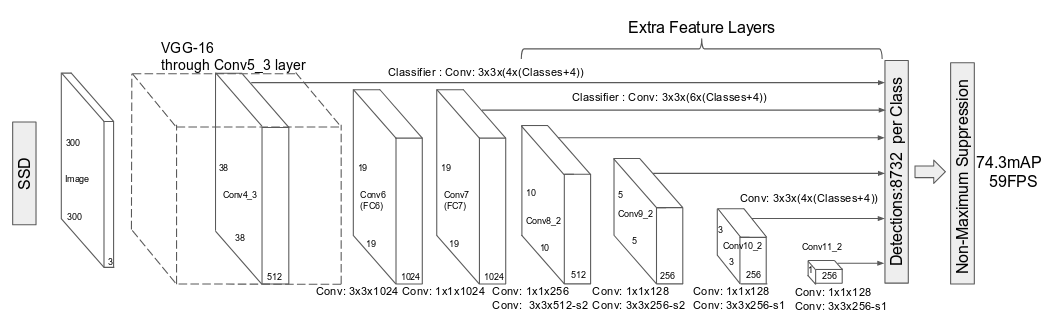
\includegraphics[width=0.9\textwidth]{3_ssd_arch.png}
	\caption[Caption for LOF]{Cấu trúc tổng quát mô hình SSD \cite{ssd}}
\end{figure}

\paragraph*{Sử dụng các bản đồ đặc trưng khác nhau cho dự đoán.} Trong cấu trúc của mạng SSD, qua các lớp tích chập, kích thước bản đồ đặc trưng giảm dần, điều này cho phép thực hiện dự đoán các đối tượng có kích thước đa dạng. Đây là khác biệt lớn nhất giữa SSD và YOLO.\\

\paragraph*{Sử dụng lớp tích chập là lớp dự đoán.} Như đã đề cập ở trên, mỗi bản đồ đặc trưng được lựa chọn vào quá trình dự đoán có thể sinh ra một tập cố định các dự đoán nhờ các bộ lọc tích chập. Ví dụ với bản đồ đặc trưng có kích thước mxn với p kênh,  sẽ sử dụng các bộ lọc có kích thước 3x3xp để có đầu ra là các điểm phân loại đối tượng và tọa độ tương đối của hộp dự đoán so với hộp mẫu.\\

\paragraph*{Số lượng hộp mặc định và tỉ lệ cạnh.} Mỗi ô trên bản đồ đặc trưng được lựa chọn để dự đoán sẽ được liên kết với một tập các hộp mặc định bằng phép tích chập. Tại mỗi ô trên bản đồ đặc trưng, SSD dự đoán vị trí tương đối của hộp tiềm năng so với hộp mặc định và điểm phân loại của mỗi nhãn/lớp mà đối tượng nằm trong hộp tiềm năng thuộc về. 
Cụ thể, tại một ô trên bản đồ đặc trưng có k hộp mặc định, chúng ta cần tính toán với bài toán có c nhãn/lớp cần phân loại và 4 tọa độ tương đối so với hộp mẫu. Kết quả sẽ có (c+4)*k bộ lọc sẽ được áp dụng lên mỗi ô trên bản đồ đặc trưng, tạo ra (c+4)*k*m*n đầu ra cho một bản đồ đặc trưng có kích thước m*n. Hình dưới minh họa    \\

\begin{figure}[h!]
	\centering
	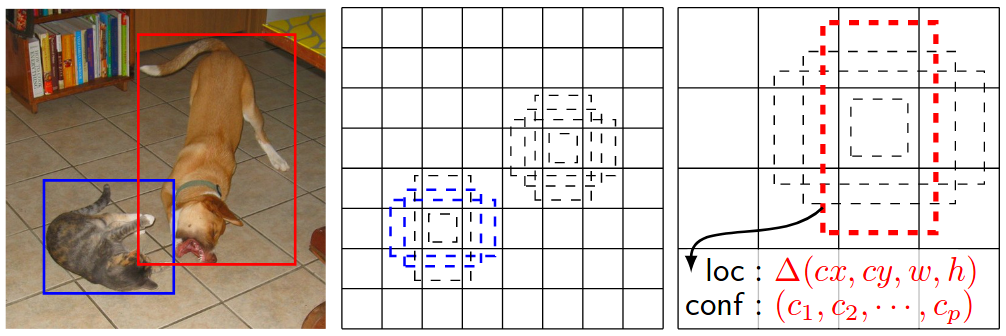
\includegraphics[width=0.9\textwidth]{3_ssd_box.png}
	\caption[Caption for LOF]{Hộp mẫu và hộp mặc định trong SSD \cite{ssd}}
	Các hộp mẫu từ ảnh (a) sẽ được gán tương ứng thành các hộp mặc định ở (b) và (c). Như vậy, thay vì phát hiện các hộp chứa tuỳ ý, SSD chỉ phát hiện một số hộp mẫu có tỉ lệ và độ lớn nhất định.  
\end{figure}

\subsubsection{Cấu trúc mạng SSD}
\begin{itemize}
\item Một framework SSD gồm có 3 phần chính: Base Model, Extra Layers, MultiBox. 
\item Base model có thể sử dụng một số mạng state-of-the-art để trích xuất đặc trưng ảnh như VGG-16, VGG-19, Resnet, AlexNet, GoogLeNet, ... Nhưng trong bản báo cáo này chỉ đề cập đến base model sử dụng mạng VGG-16.
\end{itemize}

\subsubsubsection*{Base Model - VGG-16}
\begin{table}[h]
	\caption{Cấu trúc mạng SSD300 và số lượng tham số của mỗi lớp}
	\begin{tabular}{|l|l|l|}
		\hline
		Layer & Size & Paramters \\
		(window\_size, number\_filters, stride, padding) &
		(height, width, channel)& (weights + bias)\\ \hline

		input & [300,300,3] & 0, RF = 1 \\
		& & \\ \hline
		conv\_1\_1 (3, 64, 1, 1) & [300,300,64] & 3x3x3x64 + 64 = 1792\\  
		& & RF=3, j\_out = 1 \\ \hline
		conv\_1\_2 (3, 64, 1, 1) & [300,300,64] & 3x3x64x64 + 64 = 36928 \\
		& & RF=5, j\_out = 1 \\ \hline
		pooling\_1 (2, 0, 2, 0) & [150,150,64] & 0 \\
		&&j\_out=2, RF=7 \\ \hline
		conv\_2\_1 (3, 128, 1, 1) & [150,150,128] & 3x3x64x128 + 128 = 73856\\
		&&j\_out=2, RF=11 \\ \hline
		conv\_2\_2 (3, 128, 1, 1) & [150,150,128] & 3x3x128x128 + 128 = 147584\\
		&&j\_out=2, RF=15 \\ \hline
		pooling\_2 (2, 0, 2, 0) & [75,75,128] & 0\\
		&&j\_out=4, RF=19 \\ \hline
		conv\_3\_1 (3, 256, 1, 1) & [75,75,256] & 3x3x128x256 + 256 = 295168\\
		&&j\_out=4, RF=27 \\ \hline
		conv\_3\_2 (3, 256, 1, 1) & [75,75,256] & 3x3x256x256 + 256 = 590080\\
		&&j\_out=4, RF=35 \\ \hline
		conv\_3\_3 (3, 256, 1, 1) & [75,75,256] & 3x3x256x256 + 256 = 590080\\
		&&j\_out=4, RF=43 \\ \hline
		pooling\_3 (2, 0, 2, 0) (ceil\_mode) & [38,38,256] & 0\\
		&&j\_out=8, RF=51 \\ \hline
		conv\_4\_1 (3, 512, 1, 1) & [38,38,512] & 3x3x256x512 + 512 = 1180160\\
		&&j\_out=8, RF=67 \\ \hline
		conv\_4\_2 (3, 512, 1, 1) & [38,38,512] & 3x3x512x512 + 512 = 2359808\\
		&&j\_out=8, RF=83 \\ \hline
		conv\_4\_3 (3, 512, 1, 1) & [38,38,512] & 3x3x512x512 + 512 = 2359808\\
		&& j\_out=8, RF=99 \\ \hline
		L2Norm & [38, 38, 512] & 0 \\ 
		& & \\ \hline
		pooling\_4 (2, 0, 2, 0) & [19,19,512] &0\\
		&&j\_out=16, RF=115 \\ \hline


\end{tabular}

\end{table}

\subsubsection{}
\section{Feature Fusion Single Shot MultiBox Detector}
\section{Single Shot Scale-invariant Face Detector }

\chapter{NỘI DUNG THỰC HIỆN}
\section{Mục tiêu} thử nghiệm các mô hình và giải pháp cải tiến, sau đó triển khai lên computing box
\section{Thử nghiệm các mô hình}
\subsection{Chuẩn bị dữ liệu}
\subsection{Một số tham số cần lưu ý}
\subsection{Đánh giá mô hình}
\subsection{Tối ưu hàm mất mát}

\section{Triển khai mô hình lên board Jetson}

\chapter{KẾT LUẬN, ĐÁNH GIÁ, HƯỚNG PHÁT TRIỂN}
%%%chú thích 
<abc>
\footnote{là abcd}

%%%insert ảnh, nhớ captioning và ghi nguồn 
%-------------Figure 2 ---------------------------------
%\begin{figure}[h!]
%	\centering
%	\includegraphics[width=0.8\textwidth]{anm_victim_destop2.PNG}
%	\caption{Tình trạng máy nạn nhân sau cuộc tấn công}
%	\end{figure}
	
%%%%%%%%%%%%%%%%%


%{PHỤ LỤC}
%%%%%%%%%%%%%%%%%%%%%%%%%%%%%%%%%
%\addcontentsline{\bibitem{adf}}

\begin{thebibliography}{80}
\addcontentsline{toc}{chapter}{Tài liệu tham khảo}

\bibitem{ssd}
Wei Liu, Dragomir Anguelov, Dumitru Erhan, Christian Szegedy, Scott Reed, Cheng-Yang Fu, Alexander C. Berg, "SSD: Single Shot MultiBox Detector", ECCV 2016

\bibitem{fssd}
Zuoxin Li, Fuqiang Zhou, "FSSD: Feature Fusion Single Shot Multibox Detector", arXiv 2017

\bibitem{s3sd} Shifeng Zhang, Xiangyu Zhu, Zhen Lei, Hailin Shi, Xiaobo Wang, Stan Z.Li, "S$^ 3$FD: Single Shot Scale-invariant Face Detector", ICCV 2017

\bibitem{fasterrcnn} Shaoqing Ren and Kaiming He and Ross Girshick and Jian Sun, "Faster {R-CNN}: Towards Real-Time Object Detection
with Region Proposal Networks", NIPS 2015

\bibitem{fastrcnn} Ross Girshick, "Fast{R-CNN}", ICCV 2015

\bibitem{rcnn} Ross Girshick, Jeff Donahue, Trevor Darrell, Jitendra Malik, "Rich feature hierarchies for accurate object detection and semantic segmentation", CVPR 2014 

\bibitem{dssd} RCheng-Yang Fu, Wei Liu, Ananth Ranga, Ambrish Tyagi, Alexander C. Berg, "DSSD : Deconvolutional Single Shot Detector", CVPR 2014 

\bibitem{CVX}
CVX Introduction
``\textbf{link: http://cvxr.com/cvx/doc/intro.html/}'',
\textit{What is CVX}, lần truy cập cuối: 15/04/2017.

\bibitem{detectionoverview}
Joyce Xu, Deep Learning for Object Detection: A Comprehensive Review,\\
\href {https://towardsdatascience.com/deep-learning-for-object-detection-a-comprehensive-review-73930816d8d9}{https://towardsdatascience.com/deep-learning-for-object-detection-a-comprehensive-review-73930816d8d9},

\end{thebibliography}
\end{document}

